\section{Workload Generation}

As explained in Section \ref{ch:method}, timeseries has six primary attributes. In order to create a timeseries for performance testing, it needs data for each key attribute.
While generating the timeseries for performance testing, it selected locations all over the world as a generic case to include all the locations without binding to a specific area.

These locations are taken from Google's Countries Public Data set \cite{GoogleGoogleCounties}, and consider static though out the testing, and data added to the wdias-performance-test.
During the performance test, it creates 1000 timeseries and keep adding data against those timeseries. For each location, it creates four timeseries \hl{with vary with module Id} key attribute with four values. Thus combining all together, those creates 1000 timeseries. But test cases generate these values before starts the performance tests, and able to increase the timeseries as wanted.

For grid data, it uses static 100 grid locations which based on how is \acrshort{api} exposed. Since grid locations have different metadata structure as described in \ref{se:db_struct}, those data handle separately. But the locationId of grid and scalar data types have the same effect when define a timeseries.

In the \acrshort{jmeter} Best Practices, \say{If your test needs large amounts of data - particularly if it needs to be \emph{randomised} create the test data in a file that can be read with CSV Data set. This avoids wasting resources at run-time. jmeter best practices lean\_mean}. Rather providing the randomness in run time, the timeseries stored with the random order which satisfy the percentage of 70\% Scalar, 20\% Vector and 10\% Grid as mentioned in \ref{se:test_plan}.
Before running the test cases, it generate the metadata for timeseries and write into a CSV file which is shared among the threads in the \acrshort{jmeter}. This occurs in the setup phase of the test cases. The metadata CSV file arrange in a way that within each 10 lines, 7 lines are Scalar timeseries, 2 lines are Vector timeseries, and 1 line is a Grid timeseries.

The system is capable of storing any numeric value up to 3 decimal points. It does not make any different based on the parameter type whether it is the precipitation or the temperature. Thus during the performance testing, \acrshort{jmeter} uses real precipitation data from \acrshort{curw}. One month period of data for five weather stations have been using for prepare the test data. The script to cleanup and prepare the precipitation data is available as \emph{setup\_precipitation.sh} in wdias-performance.

\begin{lstlisting}[language=sh, caption=Preparation of precipitation data.]
Set ROOT_DIR=~/wdias/wdias-performance-test
-h | --help: Usage
  setup_precipitation.sh  <COMMAND>
    - COMMAND: help | extract | prepare | cleanup | populate
  e.g.
  setup_precipitation.sh prepare
    Segregate single file data into multiple files based on date. And Separate into main directories of 15min, 30min, 60min and create tar files
  setup_precipitation.sh extract
    Extract the tar files into 15min, 30min and 60min
  setup_precipitation.sh cleanup
    Clean up extracted directories
\end{lstlisting}
When preparing the data, it create three set of data based on the time interval such as hourly (60min), 30min, and 15min data with modifying the replicated data.
This will reduce the overhead in performance testing and increase the performance itself.
Extract function use while creating the containers, and extract the data into the container. This reduce the context loading while creating the container images.
While performing the load testing, \acrshort{jmeter} keep update a date counter, and create over the one month data. At the end of current month, the date counter advance to the next month. But data is repeat using from the beginning. In order to provide more randomness, it switch over five locations as well. The JSR223 scripts were written in a generic way such that is possible to tweak and use if there are more location data available.

Almost similar to how was the precipitation data proceed, the water level are prepared for Grid data. One exception with Grid data during this test cases was, the maximum time step is 30min, instead of 15min due to larger size of the data. But the \acrshort{wdias} is capable of supporting such request. The main purpose of the \acrshort{wdias} is to provide a extensible architecture framework, during the performance testing it is not much consider about scaling the Grid data handling as it using \acrshort{netCDF}, and it is another domain with an attraction up to some extend.

\begin{lstlisting}[language=sh, caption= Preparation of water-level data.]
Set ROOT_DIR=~/wdias/wdias-performance-test
-h | --help: Usage
  setup_water-level.sh  <COMMAND>
    - COMMAND: help | extract | prepare | cleanup | populate
  e.g.
  setup_water-level.sh prepare
    Segregate single file data into multiple grid file directories based on date. And Separate into main directories of 15min, 30min, 60min and create tar files
  setup_water-level.sh extract
    Extract the tar files into 15min, 30min and 60min
  setup_water-level.sh cleanup
    Clean up extracted directories
\end{lstlisting}
The water level also contains the real data for one month of period, and \emph{setup\_waterlevel.sh} script provide the functionality of prepare, cleanup and extract.
Also it reset and repeat reading from the beginning when the \acrshort{jmeter} date counter keep increasing.


%%%%%%%%%%%%%%%%%%%%%%%%%%%%%%%%%%%%%%%%%%%%%%%%%%%%%%%%%%%%%%%%%%%%%%%%%%%%%%%%
\subsection{Experimental Setup}
In order to create higher workload using the \acrshort{jmeter}, it has Distributed Testing feature. It uses the master slave approach and it allowed to handle all the test cases via single instance, rather handling separate instances. But it has following limitation;
The same test plan runs by all the servers. JMeter does not distribute the load between servers, each runs the full test plan. So if you set 1,000 threads and have 6 JMeter server, you end up injecting 6,000 threads. When test cases runs with \acrshort{jmeter} Distributed mode, the server node trigger same copy of test case on configured slave nodes parallel. At the end of the test cases, it gather results into the master node.

\begin{figure}[htp]
    \centering
    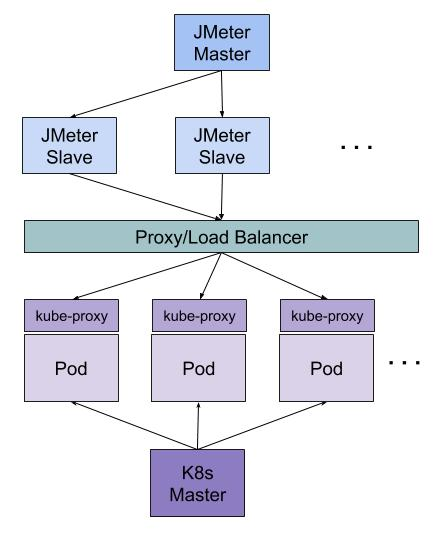
\includegraphics[width=0.6\textwidth]{results/work_load/experimental_setup_v3.jpg}
    \caption{Experimental setup with JMeter}
    \label{fi:experimental_setup}
\end{figure}

When implementing load test cases with \acrshort{jmeter}, it uses threads to simulate the users. The root component of a test create is a thread group. There are different kind of thread groups are available such as thread group (basic thread group), arrivals thread Group, free form arrivals thread group, stepping thread group, concurrency thread group, and ultimate thread group.


%%%%%%%%%%%%%%%%%%%%%%%%%%%%%%%%%%%%%%%%%%%%%%%%%%%%%%%%%%%%%%%%%%%%%%%%%%%%%%%%
\subsubsection{Closed vs. open workload models}
\label{subse:closed_vs_open_workload}
\begin{itemize}
    \item \emph{closed system model} \cite{Haggett1998AnWales} a new request is only triggered by the completion of a previous request, following by a think time. System has negative feedback that makes it impossible to bury-out the service, so users wait for the responses before making new requests.
    \item \emph{open system model} new requests arrival independently of completions, e.g.,according to a stochastic process or fixed trace. System has no negative feedback.
\end{itemize}
While implementing the test cases for \acrshort{wdias}, it uses Concurrency Thread Group with Throughput Shaping Timer because of it support the open workload approach.
Using other thread groups, it required to find exact number of threads and timer delays that produce desired number of requests per second (RPS) to server. Which is known as the \emph{closed workload}.
With using Throughput Shaping Timer, it only need to configure the \acrfull{rps}. When combine this \acrshort{jmeter} plugin with Concurrency Thread Group using Schedule Feedback Function to dynamically maintain thread count required to achieve target RPS \cite{KarunarathneGihanWdias/wdias-performance-test:JMeter.}.

The test plans mentioned in \ref{se:test_plan} are implemented via the \acrshort{jmeter}. The following list shows the all the test cases used for the performance testing:

\begin{itemize}
    \item User-defined variables
    \item Setup thread group
    \item Create timeseries thread group
    \item Create extensions thread group
    \item Load test timeseries concurrency thread group
    \item Load test timeseries concurrency thread group
    \item Test flow thread group
\end{itemize}

In the first step of the plan consist of setting up the timeseries metadata. At the same time, it creates the timeseries entry in the \acrshort{wdias} system as well as shown in following list of test steps and configurations.

\begin{itemize}
    \item HTTP request defaults
    \item HTTP header manager
    \item Timeseries metadata CSV
    \item Create timeseries
    \item Get timeseries
    \item Query timeseries
\end{itemize}

By creating the timeseries before help to reduce the overhead during the performance testing, and cause to more accurate \acrshort{rps} at the run time.
Otherwise \acrshort{jmeter} need to allocate another set of threads for timeseries creation. Since the test cases insert data again set of timeseries, most of the time it about retrieving the timeseries metadata, rather creation a new timeseries in the \acrshort{wdias} system.

Following list shows the test steps of \acrshort{jmeter} while performing the load testing and the configurations.

\begin{itemize}
    \item HTTP Request Defaults
    \item HTTP Header Manager
    \item Timeseries Metadata CSV
    \item If Scalar or Vector
        \begin{itemize}
            \item Insert Timeseries
        \end{itemize}
    \item If a Grid
    \begin{itemize}
        \item Insert Grid Timeseries
    \end{itemize}
    \item Wait for extensions timeseries
    \item Interest Area preprocessor
    \item Query If Scalar Or Vector
    \item Retrieve If Scalar or Vector
        \begin{itemize}
            \item Retrieve Timeseries
        \end{itemize}
    \item Retrieve If a Grid
    \begin{itemize}
        \item Retrieve Grid Timeseries
    \end{itemize}
    \item Increment date
    \item Throughput shaping timer prod
\end{itemize}

\hl{Following list of test steps shows intensively test the query timeseries features.}

\begin{itemize}
    \item HTTP Request Defaults
    \item HTTP Header Manager
    \item Locations CSV
    \item Interest Area preprocessor
    \begin{itemize}
        \item /Location: * → Locations
    	\item /Location: Area → Locations
    	\item /Parameter: Location → Parameters
    	\item /Parameter: Locations → Parameters
    	\item /Timeseries: Location → Timeseries
    	\item /Timeseries: Locations → Timeseries
    	\item /Timeseries: Locations, Parameter → Timeseries
    	\item /Timeseries: Area → Timeseries
    	\item /Timeseries: Area, Parameter → Timeseries
    	\item /Timeseries: *, Parameter → Timeseries
    	\item /Timeseries: * → Timeseries
	\end{itemize}
\end{itemize}

In the \ref{fi:test_prod_throughtput_shaping_timer} shows the Throughput Shaping Timer configurations for the All test case.

\begin{figure}[htp]
    \centering
    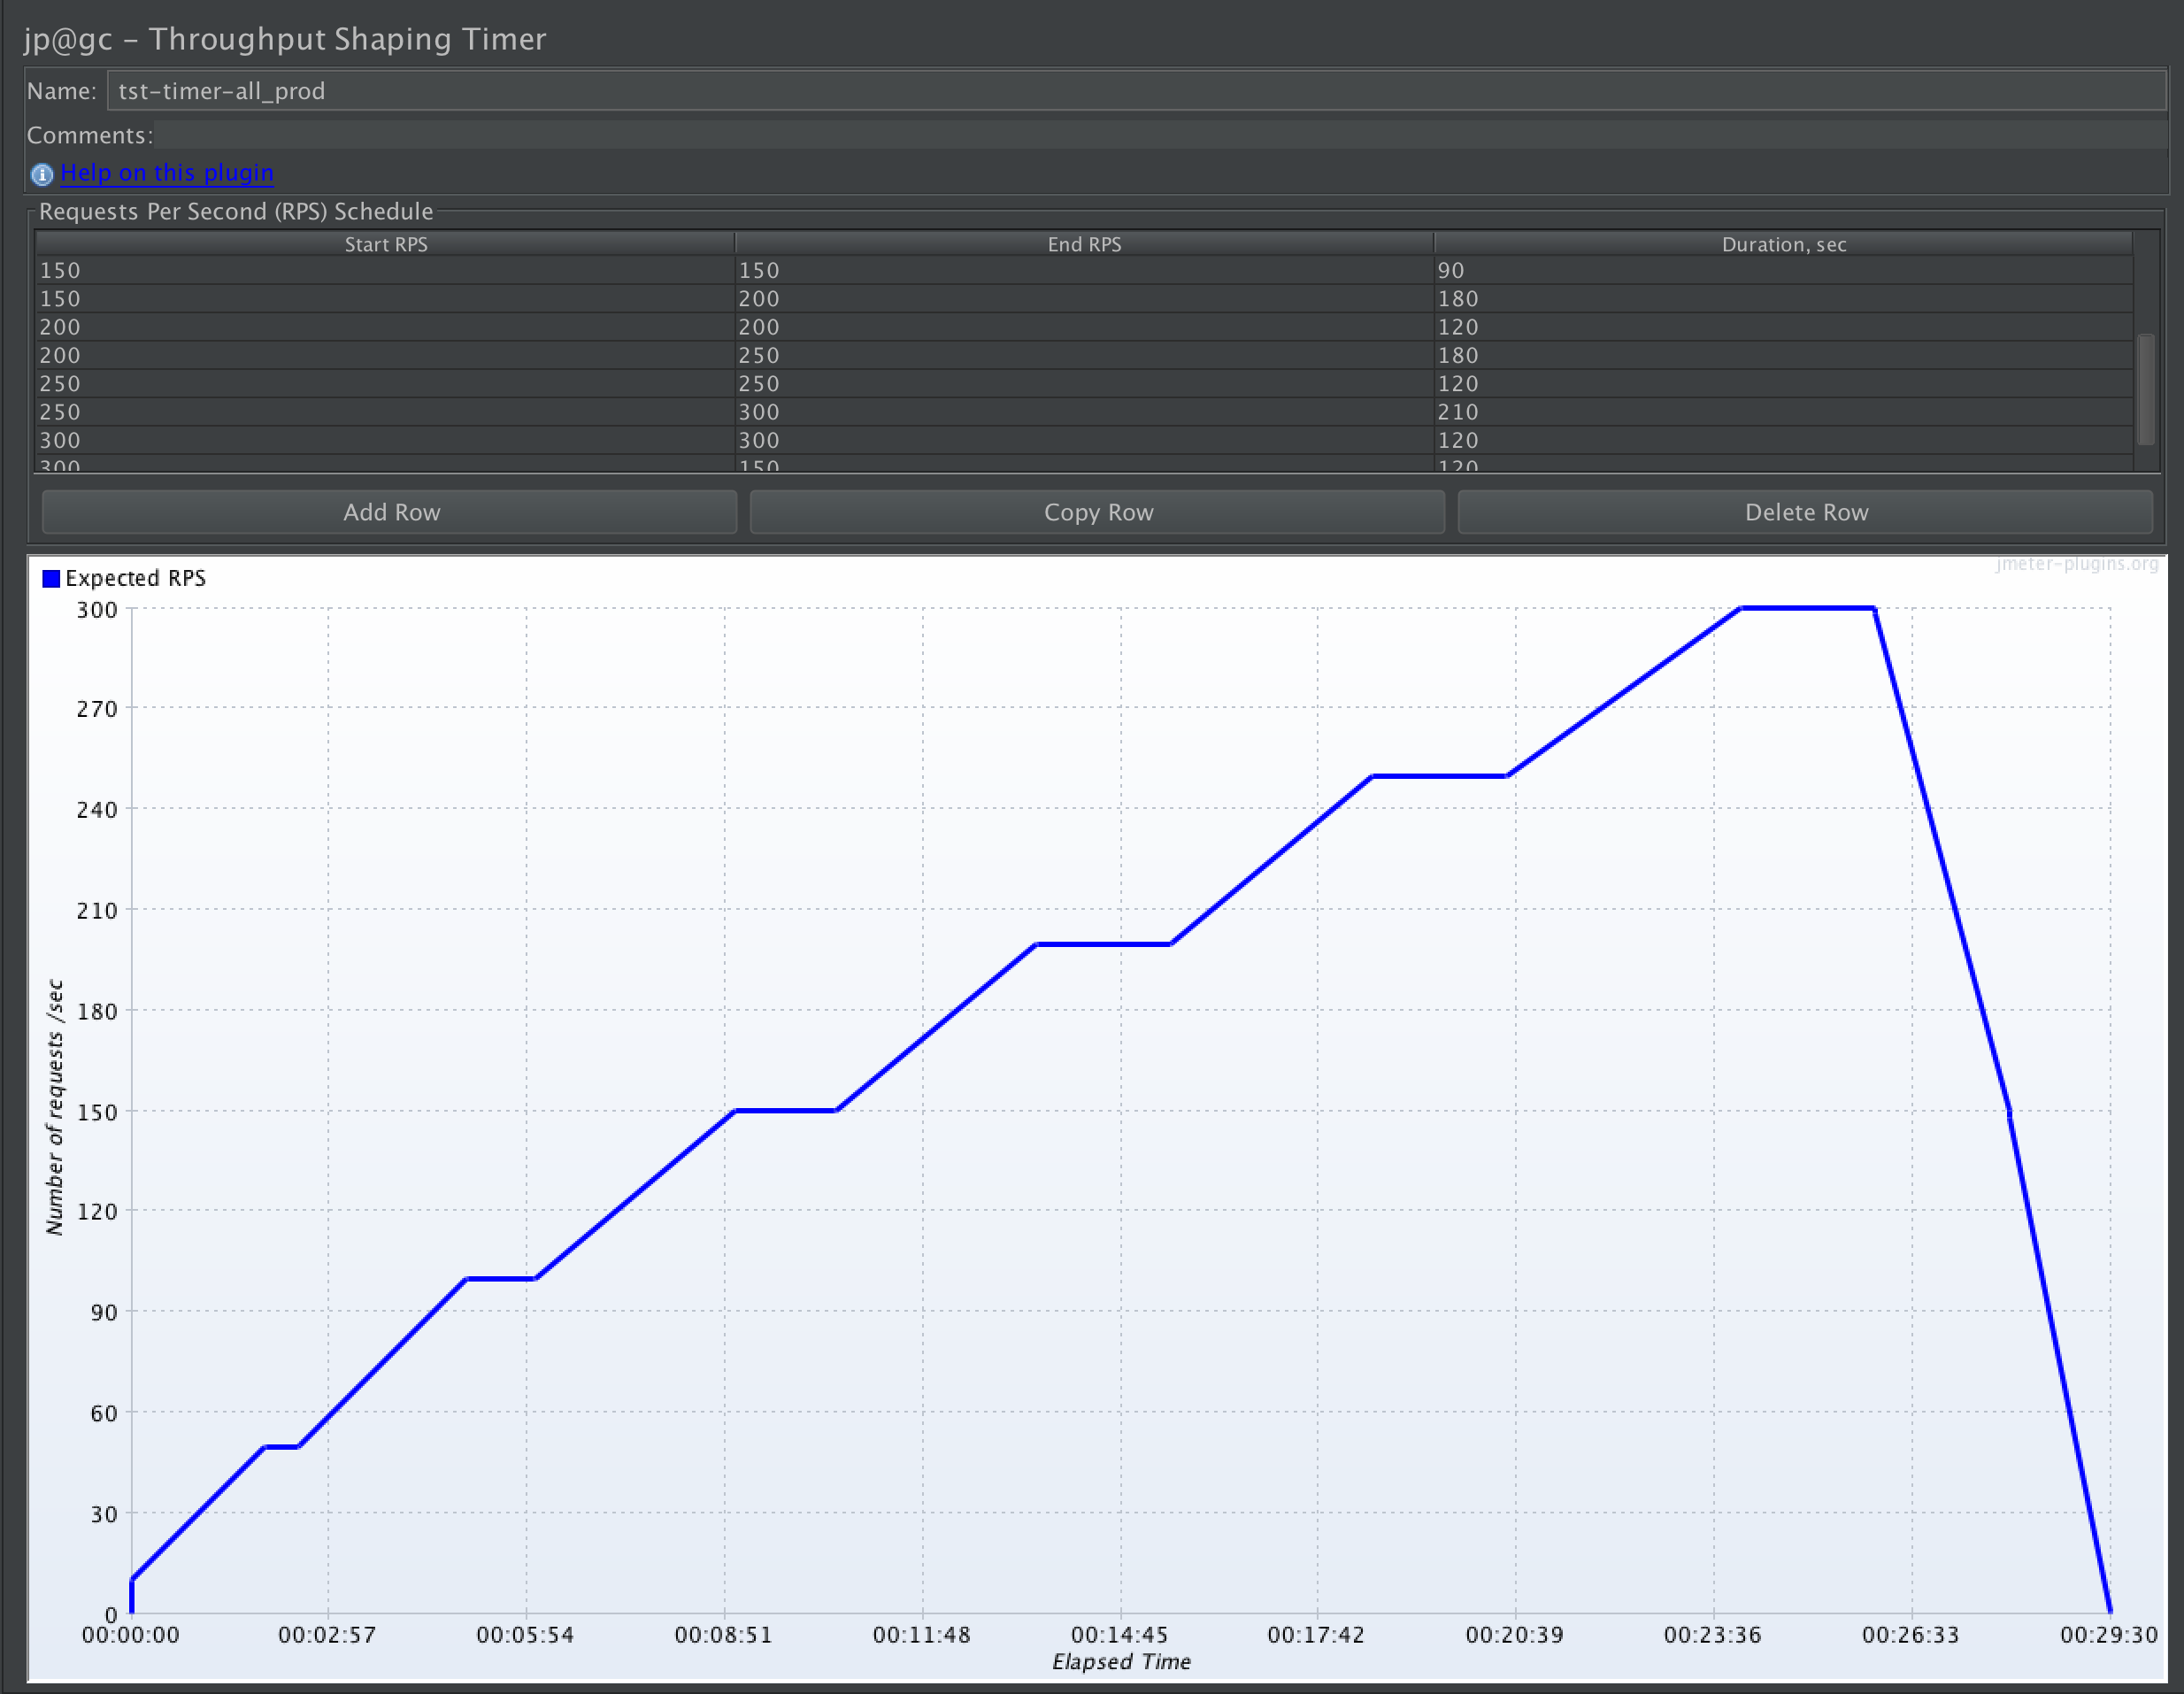
\includegraphics[width=0.6\textwidth]{results/work_load/test_prod_throughtput_shaping_timer.png}
    \caption{\acrshort{wdias} performance test - Throughput \hl{shaping timer graph}}
    \label{fi:test_prod_throughtput_shaping_timer}
\end{figure}

\dbc{Top of Fig. 4.2 useless as it's black. Anyway, this figure isn't needed}

With the above \acrshort{jmeter} test case setup, it need to enable each test case separately and before running via the command line in the server. To do it in much efficient way, a scripting tool has implemented, and accessible with the code base \cite{KarunarathneWdias-performance-test/TEST_PLAN.md:Plan} as \emph{test-dev}.

\begin{lstlisting}[language=sh, caption=Performance Test Help]
-h | --help: Usage
  test-dev enable <MODULE>
    - MODULE: import(i) | export(e) | extension(x) | all(a)

  test-dev run <REQ_SIZE>
    First need to enable module that need to be run
    - REQ_SIZE: 24(1) | 288(2) | 1440(3)
    NOTE: Modify test.conf as necessary
    e.g.
    test-dev run 24
    or
    test-dev run 1

  test-dev once <REQ_SIZE> <SEARCH_PHASE>
    This will enable the test case first. Then run the test case, and at the end disable and exit.
    - SEARCH_PHASE: Thread Group level name that matches
    e.g.
    test-dev once 24 CreateExtensions
    or
    test-dev once 1 CreateExtensions

  test-dev disable <MODULE>
    - MODULE: import(i) | export(e) | extension(x) | all(a)
\end{lstlisting}

As per the usage description of test-dev, it has the features of enable a test case, disable a test case, and run the test case while enabled.
Another wrapper was implemented around the test-dev as \emph{test-plan.sh} which is also available with the code base \cite{KarunarathneWdias-performance-test/TEST_PLAN.md:Plan}.

\begin{lstlisting}[language=sh, caption=Test Plan Help]
-h | --help: Usage
    <ROOT_DIR> <COMMAND> <REQ_SIZE>
    - COMMAND: setup | import | create_extension | extension | export | all | query
    - REQ_SIZE (optional): 24(1) | 288(2) | 1044(3)
  NOTE: Modify test.conf as necessary
  e.g.
  test_plan.sh ~/wdias/wdias-performance-test run 2
  - Run all the steps in order of setup, import, create_extension, extension, export, all, query
  test_plan.sh ~/wdias/wdias-performance-test run
  - Run all steps for all REQ_SIZE

  test_plan.sh ~/wdias/wdias-performance-test setup
  test_plan.sh ~/wdias/wdias-performance-test import 24
  test_plan.sh ~/wdias/wdias-performance-test all 24

  Distributed Mode
  SERVER_IPS=<IP1,IP2...> test_plan.sh ~/wdias/wdias-performance-test run
\end{lstlisting}

It allows to run particular test plan which are described in \ref{se:test_plan}. Also possible to run the all the test plans in order with given \emph{REQ\_SIZE} or for all the \emph{REQ\_SIZE}.

\subsubsection{JMeter performance tuning}
\begin{itemize}
    \item Use CSV files rather than random number generation
    \item Use JSR223 scripts with Groovy for data processing for test cases
    \item Using Throughput Shaping Timer to get more accurate \acrshort{rps}
\end{itemize}


%%%%%%%%%%%%%%%%%%%%%%%%%%%%%%%%%%%%%%%%%%%%%%%%%%%%%%%%%%%%%%%%%%%%%%%%%%%%%%%%
\subsection{\hl{System Configuration}}
\label{subse:test_sys_config}
As described in the \ref{se:microservice}, the \acrshort{wdias} is mainly focus on microservice architecture and implemented on top of kubernetes. \acrfull{k8s} is an open-source system for automating deployment, scaling, and management of containerized applications. For the performance study uses \acrfull{eks}. There are many \acrshort{k8s} solutions available such as GCP, Azure, and Digital Ocean on the cloud.

A detailed description of setting up the \acrshort{eks} available as \cite{KarunarathneWdias/Amazon_EKS.md:EKS} within the main repository of the \acrshort{wdias}.
\acrshort{k8s} is a planet scaling tool \cite{LinuxFoundationProduction-GradeKubernetes}, and users can tweak the configuration to run the \acrshort{wdias} as per the required level of load on the system. During the performance test of the \acrshort{wdias}, it uses maximum of 300 \acrshort{rps} with providing to the system with increasing load, and monitor the auto scalability of the system with measuring other performance parameters mentioned in Table \ref{se:test_plan}.

\begin{table}[ht]
\caption{\acrshort{eks} nodes}
\footnotesize
\begin{tabular}{lccccl}
\hline
\multicolumn{1}{c}{\textbf{Node Label}} & \textbf{vCPU} & \textbf{RAM (GB)} & \textbf{Storage (GB)} & \textbf{Quantity} & \multicolumn{1}{c}{\textbf{EC2 Name}} \\ \hline
core & 16 & 32 & 15 & 1 & c5.4xlarge \\
grid & 8 & 16 & 25 & 1 & c5.2xlarge \\
scalar & 8 & 16 & 20 & 1 & c5.2xlarge \\
test & 4 & 10.5 & 5 & 1 & c5n.xlarge \\ \hline
\end{tabular}
\label{tab:aws_eks_nodes}
\end{table}
\dbc{Center table on page}

The \acrshort{wdias} uses the Helm \cite{CNCFHelmDocs} which is a package manager for \acrshort{k8s}. Each microservice within the system deploy and maintain as a helm chart, and the Helm Charts \cite{KarunarathneWdias-helm-charts:Deployments} can be found within the code base. For the databases, it uses the official helm charts.


%%%%%%%%%%%%%%%%%%%%%%%%%%%%%%%%%%%%%%%%%%%%%%%%%%%%%%%%%%%%%%%%%%%%%%%%%%%%%%%%
\subsection{Performance Tuning}
\label{se:performance_tuning}
To get better performance using the available resources, it is possible to schedule each microservice into a predefined set of nodes. There are few ways to do in the \acrshort{k8s};
\begin{itemize}
    \item \emph{nodeSelector} -- Hard rules match for node schedule. If not match, pods will not schedule.
    \item \emph{node Affinity and Anti-Affinity} -- Soft rules for node schedule. Based on the rules, pods will schedule on most appropriate node.
    \item \emph{Taints and Tolerations} -- Opposite of nodeSelector, repel mismatching pods away from the nodes.
\end{itemize}

\begin{figure}[htp]
    \centering
    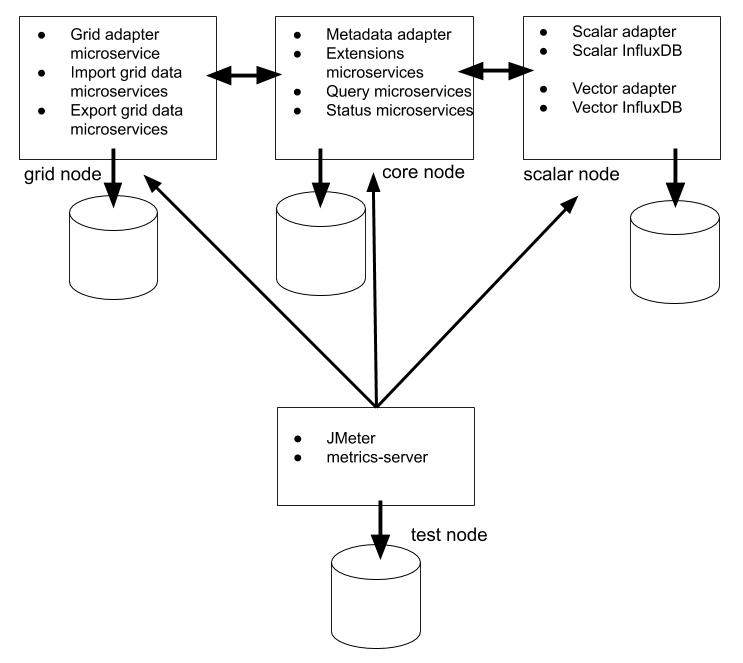
\includegraphics[width=0.75\textwidth]{results/work_load/eks_node_setup.jpg}
    \caption{\acrfull{eks} node setup}
    \label{fi:eks_node_setup}
\end{figure}

Users can use one of above features to fine-tune the \acrshort{wdias} to perform better. For the moment, \acrshort{wdias} helm charts uses node Affinity in order to use the same charts within local setup with one node and work the same charts on a \acrshort{k8s} cluster with multiple nodes. Pods are assigned to the nodes \ref{tab:aws_eks_nodes} based on the node label as below;
\begin{itemize}
    \item \emph{core} -- metadata, extensions, query, status and extension services
    \item \emph{grid} -- grid adapter, import and export grid data
    \item \emph{scalar} -- scalar and vector adapters, import and export of same data types
    \item \emph{test} -- jMeter and metric server
\end{itemize}
Figure \ref{fi:eks_node_setup} show the overview of show the nodes are setup and each microservices are assigned to each node, the connectivity of the nodes, and the data interactions via the arrows.
The databases uses for data consistency and performance in storage optimization with search capabilities. But because of that, it only possible to run one instance of those. In the \acrshort{wdias}, the MySQL and MongoDb are not getting higher load as adapter databases such as InfluxDB for scalar and vector data types, and netCDF for grid data type. In order to keep up with the pace, those microservice pods are assign to dedicated nodes in order to increase the performance of inter-service communication.
